\documentclass[11pt, oneside]{article}   	% use "amsart" instead of "article" for AMSLaTeX format
\usepackage{geometry}                		% See geometry.pdf to learn the layout options. There are lots.
\geometry{letterpaper}                   		% ... or a4paper or a5paper or ... 
%\geometry{landscape}                		% Activate for for rotated page geometry
%\usepackage[parfill]{parskip}    		% Activate to begin paragraphs with an empty line rather than an indent
\usepackage{graphicx}				% Use pdf, png, jpg, or eps� with pdflatex; use eps in DVI mode
								% TeX will automatically convert eps --> pdf in pdflatex		
\usepackage{amssymb}
\usepackage{amsmath}

\title{Two or Three quick proofs}
%\author{The Author}
%\section{}
% \subsection*{R code}
\date{}							% Activate to display a given date or no date

\graphicspath{{/Users/telliott_admin/Dropbox/Tex/png/}}

% \begin{center} 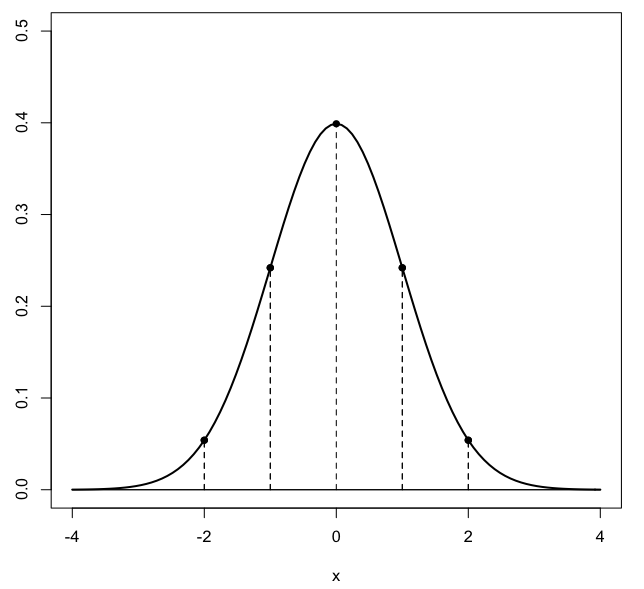
\includegraphics [scale=0.4] {gauss3.png} \end{center}
% \begin{bmatrix} a  &  b \\ c  &  d \end{bmatrix}
% \bigg |_

\begin{document}
\maketitle
\large
%\noindent

A most important fact about the exponential function $f(x) = e^x$ is that this function is its own derivative.  One way to see that is to take $\frac{d}{dx}$ of the series for $e^x$.
\[ e^x = 1 + \frac{x^{1}}{1!} + \frac{x^{2}}{2!} + \frac{x^{3}}{3!} + \cdots  \]
\[ \frac{d}{dx} \ e^x = 0 + (1)\frac{x^{1-1}}{1!} + (2)\frac{x^{2-1}}{2!} + (3)\frac{x^{3-1}}{3!} + \cdots  \]
\[ \frac{d}{dx} \ e^x = 0 + \frac{x^{0}}{0!} + \frac{x^{1}}{1!} + \frac{x^{2}}{2!} + \cdots  = e^x \]
Each exponent $n$ that comes down through the power rule, finds a term in $n! = n \times (n-1) \times (n-2) \cdots $ to cancel, leaving $n-1$ in the exponent as well as $(n-1)!$ in the denominator.

On other hand, we can also use our basic definition for the slope of the tangent to the curve $f(x)$, starting with $f(x) = b^x$
\[ \frac{d}{dx} b^x = \lim_{h \to 0} \ \frac{b^{x+h} - b^x}{h} \]
\[ = \lim_{h \to 0} \ \frac{b^{x}b^h - b^x}{h} \]
\[ = \lim_{h \to 0} \ b^{x} \frac{(b^h - 1)}{h})\]
Critically, $b^x$ does not depend on $h$ and so we can pull it out of the limit.
\[ = b^x \lim_{h \to 0} \frac{(b^h - 1)}{h})\]
The second thing is that $\lim_{h \to 0} \frac{(b^h - 1)}{h})$ is just a \emph{number}.  (Actually it turns out to be equal to $\ln(b)$).  Replace it with $k$
\[ \frac{d}{dx} b^x = k b^x \]
If we choose $b=e=2.718281828..$, then $k=1$.
\subsection*{part 2}

It is possible to obtain the definition of the derivative of the logarithm from the above.
\[ \int \frac{1}{t} \ dt = \ln(t) \]
\[ \frac{d}{dt} \int \frac{1}{t} \ dt  = \frac{1}{t}  = \frac{d}{dt} \ln(t) \]
This is great because we never did generate $x^{-1}$ by differentiating powers of $x$.  Now we know how to go back the other way.  

The proof is so simple that if you blink, you'll miss it.  Again, we found that the exponential function is its own derivative.  That is
\[ y = e^x \]
\[ \frac{d}{dx} e^x = \frac{dy}{dx} = e^x  \]
\[ \frac{dy}{dx} = y \]
Invert
\[ \frac{dx}{dy} = \frac{1}{y} \]
\[ dx = \frac{1}{y} \ dy \]
Integrate
\[ \int dx = x = \int \frac{1}{y} \ dy \]
And what is $x$?  It is $\ln(y)$!
\[ \ln(y) = \int \frac{1}{y} \ dy \]
And since $y$ is just a letter, we can write the same for $x$, or $t$
\[ \ln(t) = \int \frac{1}{t} \ dt \]
One of the prettiest things I've ever seen.

\subsection*{reverse direction}
As we said above, differentiating both sides of the last equation we get
\[ {\frac{d}{dx} \ln(x) = \frac{1}{x} } \]
We want to go backward now, to show that the derivative of the function $f(x) = e^x$ is itself.  Start with
\[ \ln(e^x) = x \]
\[ \frac{d}{dx} \ln(e^x) = \frac{d}{dx} x = 1 \]
but using the property we just proved and the chain rule, this is also
\[ \frac{d}{dx} \ln(e^x) = \frac{1}{e^x} \ \frac{d}{dx} e^x  \]
so these two expressions are equal and
\[ \frac{1}{e^x} \ \frac{d}{dx} e^x = 1  \] 
\[ \frac{d}{dx} e^x = e^x \]

\end{document}  